\documentclass[11pt]{article}

%%%%%%%%%%%%%%%%%%%%%%%%%%%%%%%%%%%%%%%%%%%%%%%%%%%%%%%%%%%%%%%%%%%%%%%%%%%%%%%%%%%%%%%%%%%%%%%%
%%%%%%%%%%%%%%%%%%%%%%%%%%%%%%%%%%%%%%%%%%%%%%%%%%%%%%%%%%%%%%%%%%%%%%%%%%%%%%%%%%%%%%%%%%%%%%%%

% MATH 167 CRN 30790
% WINTER QUARTER 2022


% Created by Xiaotie Chen, April 9th 2021

%%%%%%%%%%%%%%%%%%%%%%%%%%%%%%%%%%%%%%%%%%%%%%%%%%%%%%%%%%%%%%%%%%%%%%%%%%%%%%%%%%%%%%%%%%%%%%%%
%%%%%%%%% Load General Packages %%%%%%%%%%%%%%%%%%%%%%%%%%%%%%%%%%%%%%%%%%%%%%%%%%%%%%%%%%%%%%%%
%%%%%%%%%%%%%%%%%%%%%%%%%%%%%%%%%%%%%%%%%%%%%%%%%%%%%%%%%%%%%%%%%%%%%%%%%%%%%%%%%%%%%%%%%%%%%%%%
%%%%%%%%%%%%%%%%%%%%%%%%%%%%%%%%%%%%%%%%%%%%%%%%%%%%%%%%%%%%%%%%%%%%%%%%%%%%%%%%%%%%%%%%%%%%%%%%

\usepackage{amsmath,amssymb,amsthm,fullpage}
\usepackage{listings}
\usepackage{xcolor}
\usepackage{graphicx}
\usepackage{subfigure}

\usepackage{float}

%%%%%%%%%%%%%%%%%%%%%%%%%%%%%%%%%%%%%%%%%%%%%%%%%%%%%%%%%%%%%%%%%%%%%%%%%%%%%%%%%%%%%%%%%%%%%%%%
%%%%%%%%% Set Up Page Parameters %%%%%%%%%%%%%%%%%%%%%%%%%%%%%%%%%%%%%%%%%%%%%%%%%%%%%%%%%%%%%%%
%%%%%%%%%%%%%%%%%%%%%%%%%%%%%%%%%%%%%%%%%%%%%%%%%%%%%%%%%%%%%%%%%%%%%%%%%%%%%%%%%%%%%%%%%%%%%%%%

% Please refer to Prof. Puckett 's template for explanations

\setlength{\textheight}{ 620 pt}
\setlength{\voffset}{-20 pt}
\setlength{\headsep}{12 pt}
\setlength{\headheight}{14 pt}
\setlength{\topskip}{12 pt}
\setlength{\footskip}{30 pt}
\setcounter{MaxMatrixCols}{20}

%%%%%%%%%%%%%%%%%%%%%%%%%%%%%%%%%%%%%%%%%%%%%%%%%%%%%%%%%%%%%%%%%%%%%%%%%%%%%%%%%%%%%%%%%%%%%%%%
%%%%%%%% SET HEADERS AND FOOTERS %%%%%%%%%%%%%%%%%%%%%%%%%%%%%%%%%%%%%%%%%%%%%%%%%%%%%%%%%%%%%%%
%%%%%%%%%%%%%%%%%%%%%%%%%%%%%%%%%%%%%%%%%%%%%%%%%%%%%%%%%%%%%%%%%%%%%%%%%%%%%%%%%%%%%%%%%%%%%%%%
% "L" stands for "Left", "C" for "Centered", "R" for "Right", "O" for Odd and "E" for Even page

\usepackage{fancyhdr}
\pagestyle{fancy}
\fancyhead{}

\fancyhead[L]{\textbf{NAME: Ishita Dutta}} % TYPE YOUR NAME HERE!
\fancyhead[C]{\textbf{HW 01}}              % TYPE THE ASSGNMENT NAME HERE!
\fancyhead[R]{\textbf{SID: 918193342}}     % TYPE YOUR STUDENT ID HERE!

\fancyfoot[L]{CRN 38665}
\fancyfoot[C]{--~\thepage~--}
\fancyfoot[R]{\today}

%%%%%%%%%%%%%%%%%%%%%%%%%%%%%%%%%%%%%%%%%%%%%%%%%%%%%%%%%%%%%%%%%%%%%%%%%%%%%%%%%%%%%%%%%%%%%%%%
%%%%%%%% START DOCUMENT
%%%%%%%%%%%%%%%%%%%%%%%%%%%%%%%%%%%%%%%%%%%%%%%%%%%%%%%%%%%%%%%%%%%%%%%%%%%%%%%%%%%%%%%%%%%%%%%%

\begin{document}

 % Create a numbered list

 \begin{enumerate}

%%%%%%%%%%%%%%%%%%%%%%%%%%%%%%%%%%%%%%%%%%%%%%%%%%%%%%%%%%%%%%%%%%%%%%%%%%%%%%%%%%%%%%%%%%%%%%%%
 %%%%%%%% Problem 1
%%%%%%%%%%%%%%%%%%%%%%%%%%%%%%%%%%%%%%%%%%%%%%%%%%%%%%%%%%%%%%%%%%%%%%%%%%%%%%%%%%%%%%%%%%%%%%%%

    % Always indent your code whether it's LaTeX or Matlab. It make is easier and clearer to
    % read, and this leads to fewer mistakes. I always use 2 spaces. I think Overleaf uses
    % 4 spaces for LaTeX code.

    \item \label{Problem_01} (30 pts)

      % Create a list at the inside Problem 01. By default it will be labeled with lowercase
      % letters (a), (b) ...

      \begin{enumerate}
      
        \item a)
        $$ D = 
        \begin{bmatrix} 
        0 & 1 & 0 & 0 & 1 & 1 & 0 & 0 & 0 & 0 & 0 \\
        0 & 0 & 0 & 1 & 0 & 0 & 0 & 0 & 0 & 1 & 0 \\
        0 & 1 & 0 & 0 & 0 & 0 & 0 & 1 & 0 & 0 & 0 \\
        0 & 0 & 1 & 1 & 0 & 0 & 0 & 0 & 0 & 0 & 0 \\
        0 & 0 & 0 & 1 & 0 & 0 & 0 & 0 & 0 & 1 & 0 \\
        1 & 1 & 0 & 0 & 0 & 0 & 0 & 0 & 0 & 0 & 1 \\
        0 & 0 & 0 & 0 & 0 & 0 & 1 & 0 & 0 & 0 & 0 \\
        0 & 0 & 1 & 0 & 0 & 0 & 0 & 0 & 1 & 0 & 0 
        \end{bmatrix}$$
        
        \vskip 06pt
        \item b)
        $$\mathbf{q} = \begin{bmatrix} 0 \\ 1 \\ 0 \\ 1 \\ 0 \\ 0 \\ 0 \\ 0 \end{bmatrix}$$

        \vskip 06pt
        \item c)
        With 1-norm, you get:
        $$
        \mathbf{qd}_1 = \begin{bmatrix} 3 & 5 & 2 & 1 & 3 & 3 & 3 & 3 & 3 & 2 & 3 \end{bmatrix}
        $$
        2-norm basically taking the root for all of these numbers:
        $$
        \mathbf{qd}_2 = \begin{bmatrix} \sqrt{3} & \sqrt{5} & \sqrt{2} & \sqrt{1} & \sqrt{3} & \sqrt{3} & \sqrt{3} & \sqrt{3} & \sqrt{3} & \sqrt{2} & \sqrt{3} \end{bmatrix}
        $$
        Max-norm:
        $$
        \mathbf{qd}_{\mathrm{max}} = \begin{bmatrix} 1 & 1 & 1 & 1 & 1 & 1 & 1 & 1 & 1 & 1 & 1 \end{bmatrix}
        $$
        Using these numbers I find documents 4, 3, and 10 (in order) most useful for this seach. I would use the 1-norm method as it is most simple as well as properly informative in this case. 
        
      \end{enumerate}



%%%%%%%%%%%%%%%%%%%%%%%%%%%%%%%%%%%%%%%%%%%%%%%%%%%%%%%%%%%%%%%%
 %%%%%%%% Problem 2
%%%%%%%%%%%%%%%%%%%%%%%%%%%%%%%%%%%%%%%%%%%%%%%%%%%%%%%%%%%%%%%%%%%%%%%%%%%%%%%%%%%%%%%%%%%%%%%%

    \item \label{Problem_02} (15 pts)

        \begin{enumerate}

             \item 
             $$
             A = 
             \begin{bmatrix} 
             a_{\mathrm{11}} & a_{\mathrm{12}} &  \cdots & a_{\mathrm{1n}} \\
             a_{\mathrm{21}} & a_{\mathrm{22}} &  \cdots & a_{\mathrm{2n}} \\
             \vdots & \ddots & \vdots \\
             a_{\mathrm{m1}} & a_{\mathrm{m2}} &  \cdots & a_{\mathrm{mn}} 
             \end{bmatrix}
             $$
             \vskip 03pt
             $$
             B = 
             \begin{bmatrix} 
             b_{\mathrm{11}} & b_{\mathrm{12}} &  \cdots & b_{\mathrm{1m}} \\
             b_{\mathrm{21}} & b_{\mathrm{22}} &  \cdots & b_{\mathrm{2m}} \\
             \vdots & \ddots & \vdots \\
             b_{\mathrm{n1}} & b_{\mathrm{n2}} &  \cdots & b_{\mathrm{nm}} 
             \end{bmatrix}
             $$
             \vskip 03pt
             $$
             AB = 
             \begin{bmatrix} 
             \mathbf{a}_{\mathrm{1.}}*\mathbf{b}_{\mathrm{.1}} & \mathbf{a}_{\mathrm{1.}}*\mathbf{b}_{\mathrm{.2}} &  \cdots & \mathbf{a}_{\mathrm{1.}}*\mathbf{b}_{\mathrm{.m}} \\
             \mathbf{a}_{\mathrm{2.}}*\mathbf{b}_{\mathrm{.1}} & \mathbf{a}_{\mathrm{2.}}*\mathbf{b}_{\mathrm{.2}} &  \cdots & \mathbf{a}_{\mathrm{2.}}*\mathbf{b}_{\mathrm{.m}} \\
             \vdots & \ddots & \vdots \\
             \mathbf{a}_{\mathrm{m.}}*\mathbf{b}_{\mathrm{.1}} & \mathbf{a}_{\mathrm{m.}}*\mathbf{b}_{\mathrm{.2}} &  \cdots & \mathbf{a}_{\mathrm{m.}}*\mathbf{b}_{\mathrm{.m}}
             \end{bmatrix}
             $$
             \vskip 03pt
             $$
             BA = 
             \begin{bmatrix} 
             \mathbf{b}_{\mathrm{1.}}*\mathbf{a}_{\mathrm{.1}} & \mathbf{b}_{\mathrm{1.}}*\mathbf{a}_{\mathrm{.2}} &  \cdots & \mathbf{b}_{\mathrm{1.}}*\mathbf{a}_{\mathrm{.n}} \\
             \mathbf{b}_{\mathrm{2.}}*\mathbf{a}_{\mathrm{.1}} & \mathbf{b}_{\mathrm{2.}}*\mathbf{a}_{\mathrm{.2}} &  \cdots & \mathbf{b}_{\mathrm{2.}}*\mathbf{a}_{\mathrm{.n}} \\
             \vdots & \ddots & \vdots \\
             \mathbf{b}_{\mathrm{n.}}*\mathbf{a}_{\mathrm{.1}} & \mathbf{b}_{\mathrm{n.}}*\mathbf{a}_{\mathrm{.2}} &  \cdots & \mathbf{b}_{\mathrm{n.}}*\mathbf{a}_{\mathrm{.n}}
             \end{bmatrix}
             $$
             \vskip 0.3pt
             $$
             tr(AB) = \mathbf{a}_{\mathrm{1.}}*\mathbf{b}_{\mathrm{.1}} + \mathbf{a}_{\mathrm{2.}}*\mathbf{b}_{\mathrm{.2}} + . . . + \mathbf{a}_{\mathrm{m.}}*\mathbf{b}_{\mathrm{.m}}
             $$
             $$
             tr(BA) = \mathbf{b}_{\mathrm{1.}}*\mathbf{a}_{\mathrm{.1}} + \mathbf{b}_{\mathrm{2.}}*\mathbf{a}_{\mathrm{.2}} + . . . + \mathbf{b}_{\mathrm{n.}}*\mathbf{a}_{\mathrm{.n}}
             $$ 
             In the end, we would be multiplying the same numbers in a similar order then summing them up, which makes it so that tr(AB) = tr(BA).

             \vskip 06pt
             \item b)
             tr(AB) = 1 + 4 + 9 + 16 + 25 = 55

        \end{enumerate}

   %%%%%%%%%%%%%%%%%%%%%%%%%%%%%%%%%%%%%%%%%%%%%%%%%%%%%%%%%%%%%%%%%%%%%%%%%%%%%%%%%%%%%%%%%%%%%%%%
 %%%%%%%% Problem 3
%%%%%%%%%%%%%%%%%%%%%%%%%%%%%%%%%%%%%%%%%%%%%%%%%%%%%%%%%%%%%%%%%%%%%%%%%%%%%%%%%%%%%%%%%%%%%%%%

    \item \label{Problem_03} (50 pts)


        %%%%%%%%%%%%%%%%%%%%%%%%%%%%%%%%%%%%%%%%%%%%%%%%%%%%%%%%%%%%%%%%%%%%%%%%%%%%%%%%%%%%%%%%%%%%%%%%
 %%%%%%%% Problem 4
%%%%%%%%%%%%%%%%%%%%%%%%%%%%%%%%%%%%%%%%%%%%%%%%%%%%%%%%%%%%%%%%%%%%%%%%%%%%%%%%%%%%%%%%%%%%%%%%

    \item \label{Problem_04} (50 pts)

      \begin{enumerate}

        \item a)
        $$
        T(\mathbf{v}) = A(\mathbf{v})
        $$
        $$
        \hskip 30pt = \begin{bmatrix} 1 & 2 & 1 \\
        3 & 4 & 2 \\
        4 & 8 & 4 \\
        4 & 6 & 3
        \end{bmatrix} * \begin{bmatrix} v1 \\ v2 \end{bmatrix}
        $$
        $$
        \hskip 30pt = \begin{bmatrix} 1 & 2 \\
        0 & -2 \\
        0 & 0 \\
        0 & 0
        \end{bmatrix} * \begin{bmatrix} v1 \\ v2 \end{bmatrix}
        $$
        $$
        \hskip 30pt = \begin{bmatrix} v1 & 2v2 \\
        0 & -2v2 \\
        0 & 0 \\
        0 & 0
        \end{bmatrix}
        $$

        \vskip 06pt
        \item b)
        $$
        C(A) = \begin{bmatrix} 1 \\ 3 \\ 4 \\ 4 \end{bmatrix} , \begin{bmatrix} 0 \\ -2 \\ 0 \\ -2 \end{bmatrix}
        $$

        \vskip 06pt
        \item c) The nullspace is the inverse image of the zero vector of A; the set of vectors such that Tv = 0 for all v in null(T).

        \vskip 06pt
        \item d)
        $$
        C(A) = \begin{bmatrix} 0 \\ -1/2 \\ 1 \end{bmatrix}
        $$

        \vskip 06pt
        \item e) The row space of a matrix is the collection of all of its linear combinations of the rows. Essentially separate the matrix on the rows, and each row is its separate vector to get the row space of a matrix. Replace row with column for the column space. 

        \vskip 06pt
        \item f)
        $$
        C(A^{T}) = \begin{bmatrix} 1 & 0 & 0 \\  0 & 1 & 1/2 \end{bmatrix}
        $$
        
        \vskip 06pt
        \item g) The left nullspace is the inverse image of the zero vector of A(T), the set of vectors such that A(T)v = 0.
        
        \vskip 06pt
        \item h)
        $$
        N(A^{T}) = \begin{bmatrix} 1 & 0 & -1/4 & 0 \\ 0 & 1 & 1/4 & -1 \end{bmatrix}
        $$

        \vskip 06pt
        \item i) $$ rank(A) = 2$$

      \end{enumerate}

%%%%%%%%%%%%%%%%%%%%%%%%%%%%%%%%%%%%%%%%%%%%%%%%%%%%%%%%%%%%%%%%
 %%%%%%%% Problem 5
%%%%%%%%%%%%%%%%%%%%%%%%%%%%%%%%%%%%%%%%%%%%%%%%%%%%%%%%%%%%%%%%%%%%%%%%%%%%%%%%%%%%%%%%%%%%%%%%

    \item \label{Problem_05} (25 pts)

      \begin{enumerate}

        \item a)
        A linearly independent set must have no free rows when reduced to row echelon form. This means that after reaching row echelon form, there should not be any rows where the row is:
        $$ \mathbf{r}_x = \begin{bmatrix} 0 & 0 & \cdots & 0 \end{bmatrix} $$

        \vskip 06pt
        \item 
        Based on the definition above:
        $$
        B = 
        \begin{bmatrix} 1 & 2 & 1 \\ 0 & 1 & -1 \\ 0 & 0 & 2 \end{bmatrix}
        $$
        Because there are no rows where the entire row is all 0s, we can conclude this set is linearly independent.
        
      \end{enumerate}

%%%%%%%%%%%%%%%%%%%%%%%%%%%%%%%%%%%%%%%%%%%%%%%%%%%%%%%%%%%%%%%%
 %%%%%%%% Problem 6
%%%%%%%%%%%%%%%%%%%%%%%%%%%%%%%%%%%%%%%%%%%%%%%%%%%%%%%%%%%%%%%%%%%%%%%%%%%%%%%%%%%%%%%%%%%%%%%%

    \item \label{Problem_06} (70 pts)


             
             \graphicspath{ {.} }
             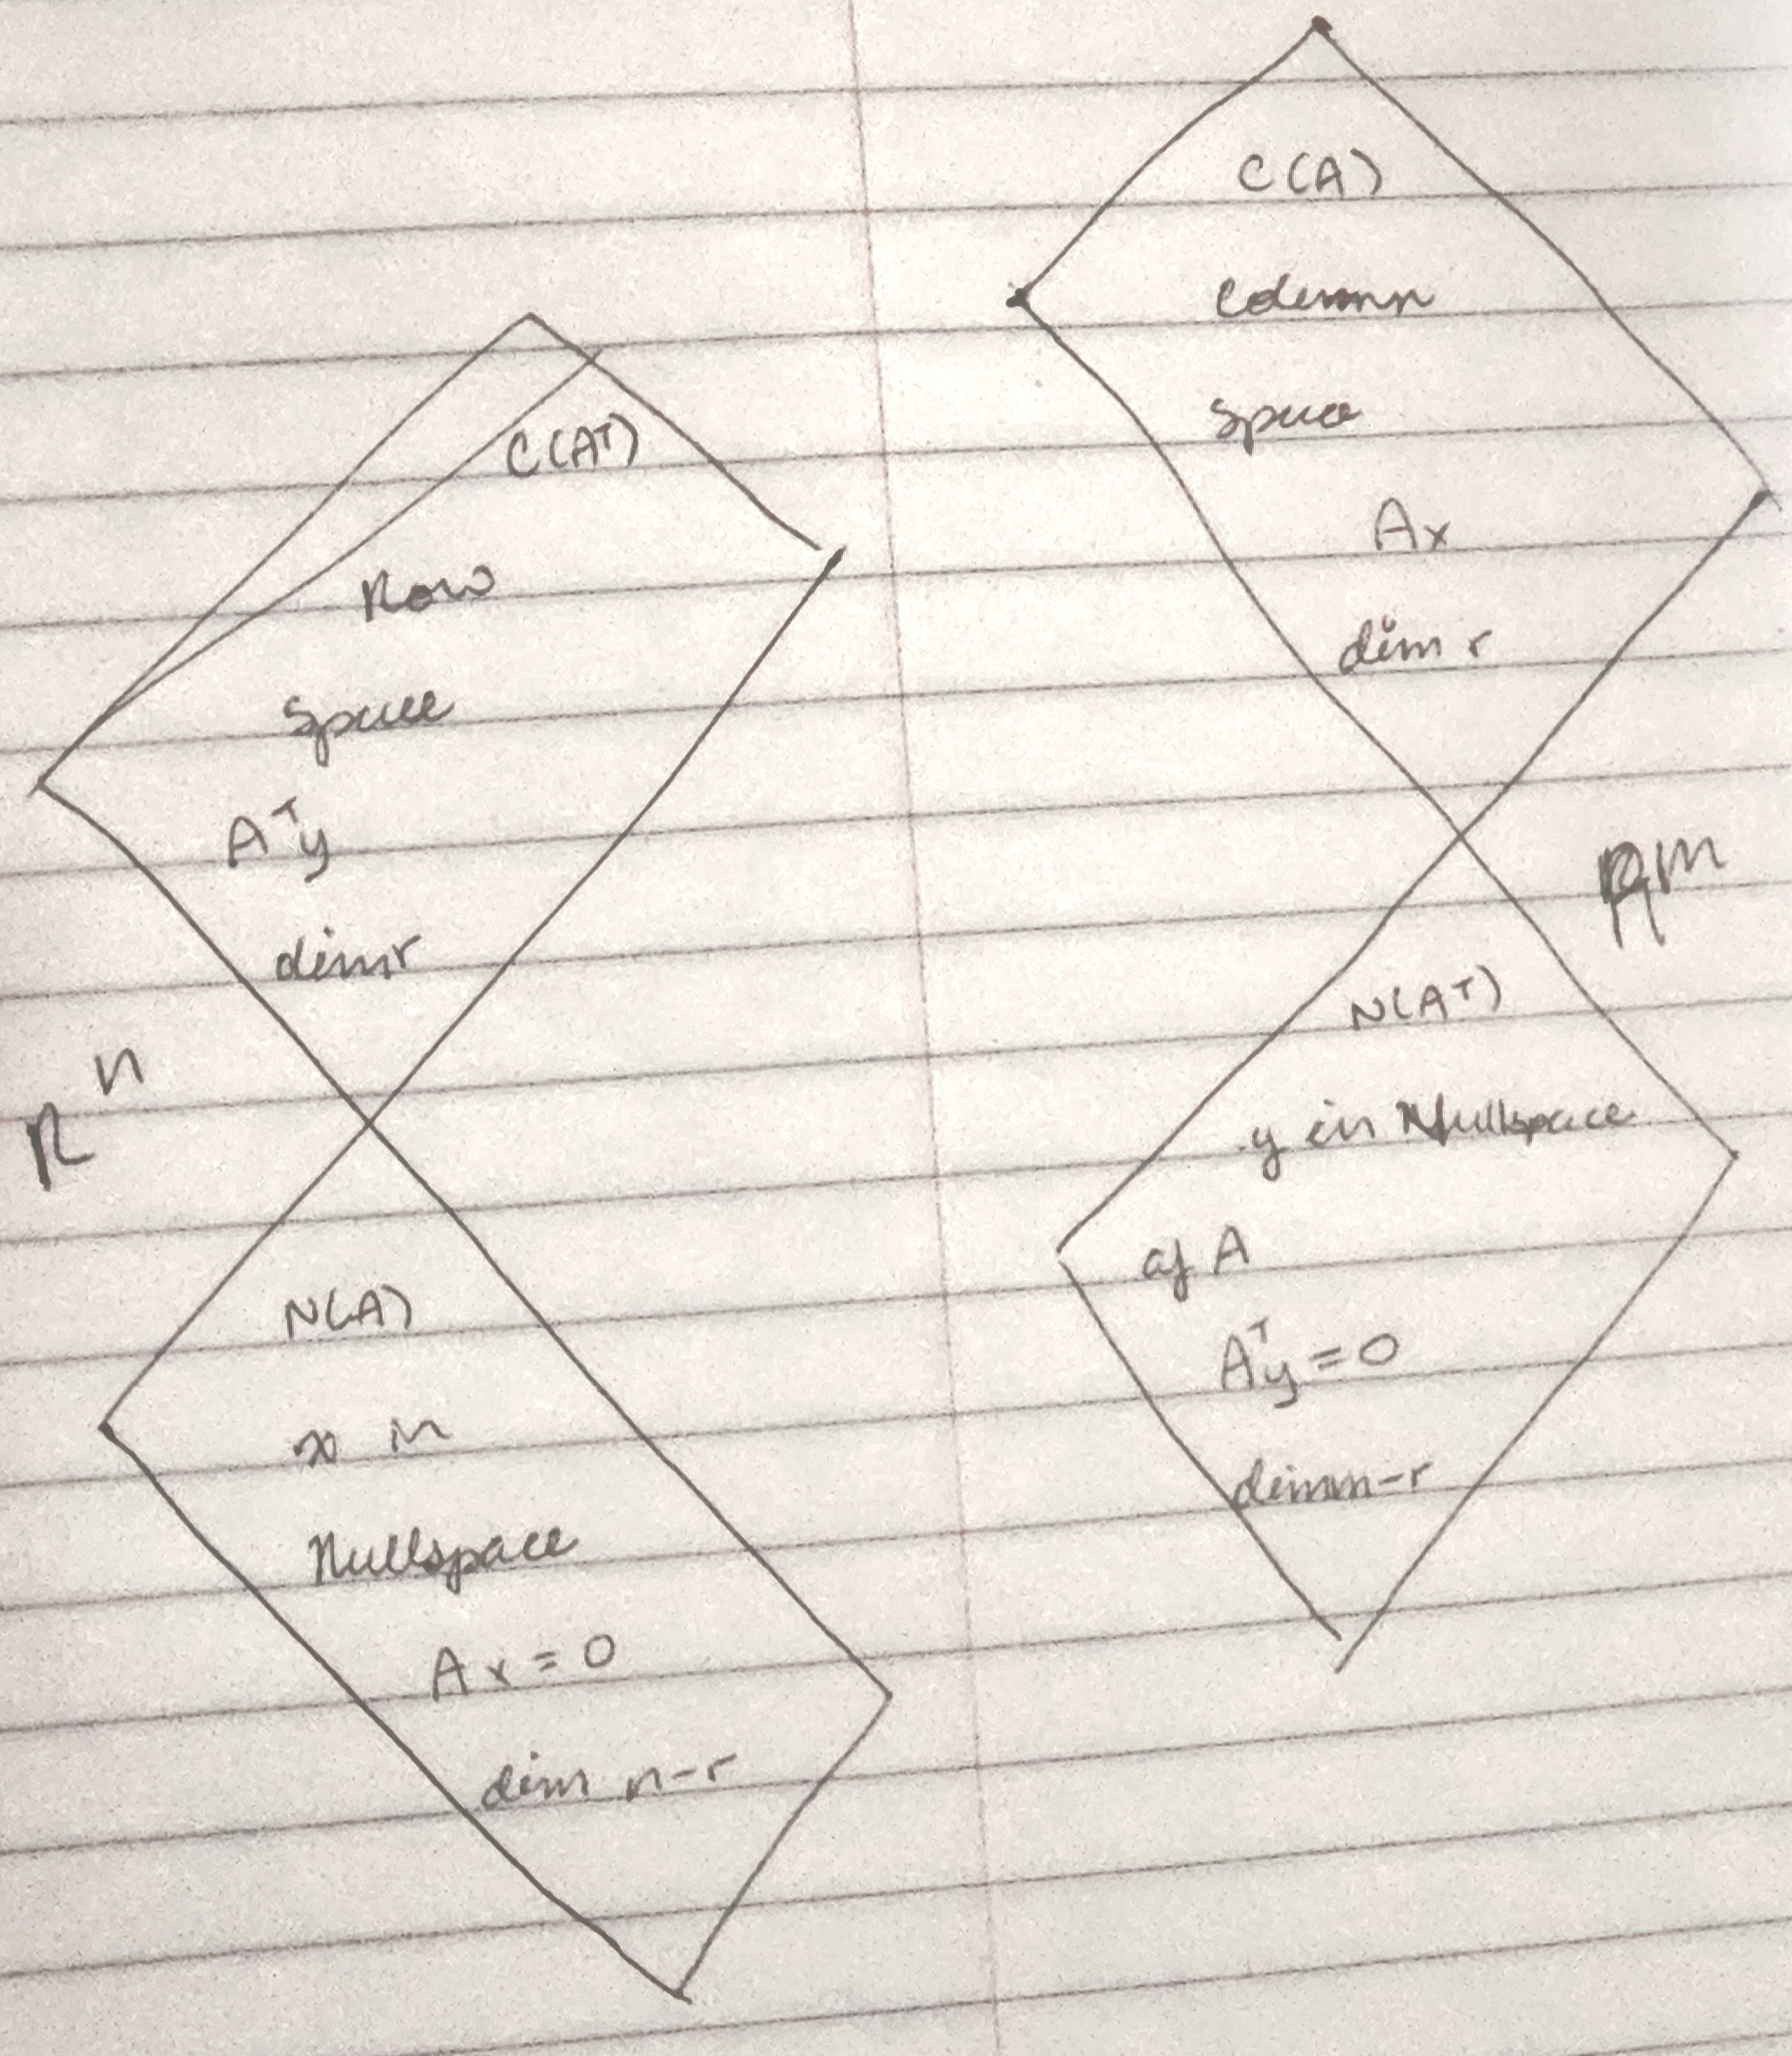
\includegraphics[width=12cm, height=18cm]{hw1q6.jpg}





\end{enumerate}

\end{document}